\chapter{Trees reveal the importance of measures in SLZ} \label{ch:revealing_trees}

%--------------------------
\section{Introduction} \label{sec:bagging_intro}
%--------------------------

The MDS analysis presented in Chapter~\ref{ch:acousticlandscape} provides us an understanding of the acoustic shape that voice quality takes in SLZ. This shape is defined by different dimensions that correspond to the glottal configuration needed to produce each voice quality and the amount of noise in the signal. The MDS analysis also provides us with a way to visualize how the different voice qualities occupy an acoustic space. Finally, the chapter discussed how different acoustic measures are correlated with different dimensions of the acoustic space. This provides us with a potential avenue to explore which measures contribute to our understanding of the different voice qualities in SLZ.
However, the analysis does not tell us which measures are the most important in making the splits between the different voice qualities. This is where decision trees are helpful as they provide a way to cut through the noise and reveal which measures play the most important role in dividing that acoustic space. 

In this chapter, I present an analysis using a flavor of decision trees called Random Forests \citep{breimanClassificationRegressionTrees1986,breimanRandomForests2001}. Random Forests are a type of ensemble learning method that combines multiple decision trees that are built on the same data. This allows us to take advantage of the strengths of decision trees while minimizing the weaknesses that are present in classical decision trees (see \cite{hastieElementsStatisticalLearning2009,boehmkeHandsOnMachineLearning2019,jamesIntroductionStatisticalLearning2021} for a discussion of the strengths and weaknesses of the different types of decision trees).

In this chapter, I show that only a small number of acoustic measures are needed to classify the different voice qualities and make the splits in the acoustic space. 

%--------------------------
\section{What are Decision Trees} \label{sec:what_are_dt}
%--------------------------

Decision trees are a statistical tool that helps to reveal which predictors divide the space under investigation. Essentially, this is done by stratifying or segmenting the predictor space into some number of simpler regions. The rules that divide the space into these regions are based on some aspect of the predictors (see \cite{hastieElementsStatisticalLearning2009,jamesIntroductionStatisticalLearning2021} for explanations of the statistics and how to perform these analyzes in R). 

These trees can be used for both regression and classification. In the case of regressions, it splits the predictor space into regions and calculates how the item under discussion behaves in each region. This process of splitting into regions and calculating how something responds in that region continues until some stopping rule is applied, which is usually defined to some number of terminal nodes. This resulting tree is rather large and is then pruned based on the cost-complexity pruning to a subset of itself. This subsetted tree is the tree that has minimized its cost-complexity criterion for all potential subsets. That is, it balances the trade-off between the complexity of the tree and its fit to the data. 

In the case of classification, the algorithms that result in a tree are very similar to those used for regression trees. The main difference in the algorithm comes from what is used to split the nodes and how the tree is pruned. Instead of predicting a continuous outcome like with regression trees, classification trees predict a categorical outcome. The predictor space is divided into regions and within each region, the majority class is assigned as the predicted class for that region. This process continues until a stopping rule is applied, similar to regression trees. The resulting tree can also be pruned to avoid overfitting, using a cost-complexity criterion.

Decision trees are easy to interpret and visualize, making them an ideal choice for understanding the structure of data and how the different predictors interact with data \citep{hastieElementsStatisticalLearning2009,jamesIntroductionStatisticalLearning2021}.

%-----------------------------
\section{Decision trees in linguistics}\label{sec:dt_linguistics}
%-----------------------------

The use of decision trees in linguistics is not new. One of the first uses was done by \citet{tagliamonteModelsForestsTrees2012}, where they illustrated the use of decision trees in investigating which sociolinguistic factors were the most important in the use of \textit{was} versus \textit{were} in York English. 

Recently, decision trees were used to show which acoustic measures were important in making the split in the acoustic space for voice quality \citep{keatingCrosslanguageAcousticSpace2023}. \citeauthor{keatingCrosslanguageAcousticSpace2023} performed a simple decision tree analysis to supplement their MDS analysis of voice quality in 11 languages. The results of this analysis are shown in Figure~\ref{fig:keating_tree}. Decision trees like the one in Figure~\ref{fig:keating_tree}, show the binary splits that are made in the space and what predictor, and the value of that predictor, makes that split. In the case of \citeauthor{keatingCrosslanguageAcousticSpace2023}'s (\citeyear{keatingCrosslanguageAcousticSpace2023}) tree, the first split is made on the harmonics-to-noise ratio over the frequency range from 0 to 500 Hz for the middle third of each vowel. This split is made at the z-score of 0.48. If the predictor value is greater than or equal to 0.48, the dominant voice quality of that region is modal. If HNR < 500 Hz value is less than 0.48, the region needs to be further split. 

\begin{figure}[h!]
    \centering
    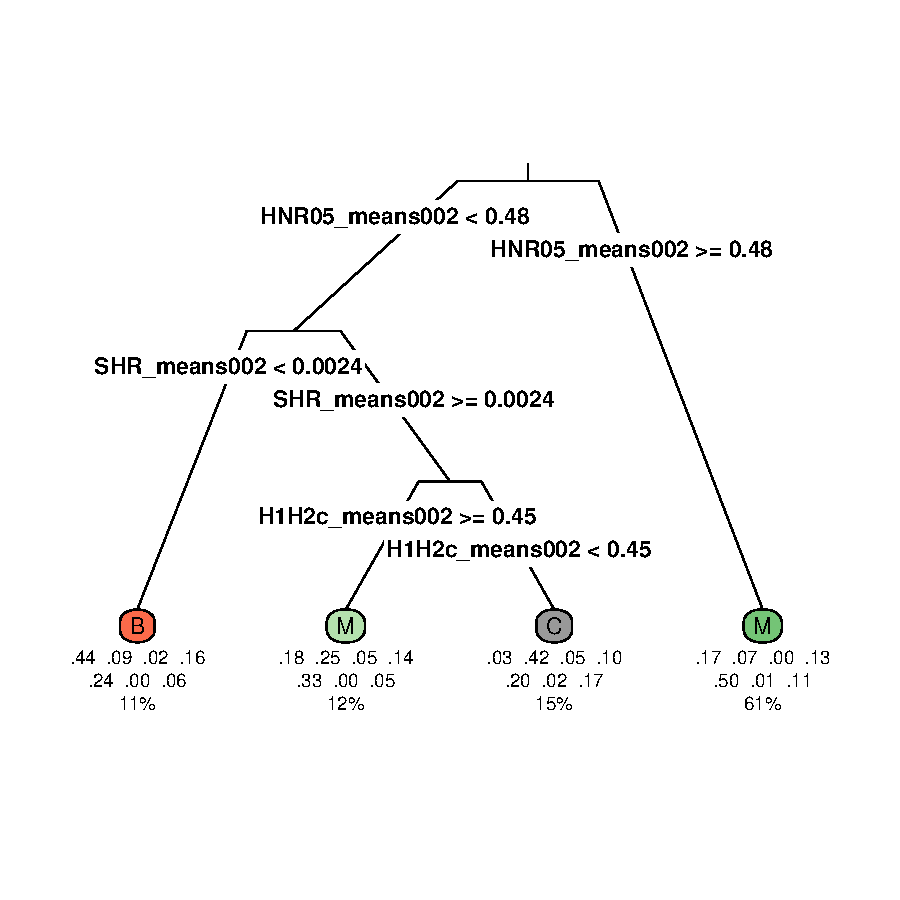
\includegraphics[width = 0.9\linewidth]{images/keating_tree.pdf}
    \caption{Classification tree of phonation categories from \citet{keatingCrosslanguageAcousticSpace2023}. Abbreviations used in this figure are: {HNR05_means002}: harmonics-to-noise ratio over the frequency range from 0 Hz to 500 Hz for the middle third of each vowel; {SHR_means002}: subharmonic-to-harmonic ratio for the middle third of each vowel; {H1H2c_means002}: H1* − H2* for the middle third of each vowel; B: breathy, M: modal, and C: creaky phonation categories.}
    \label{fig:keating_tree}
\end{figure}

The next split in the region is made on the subharmonic-to-harmonic ratio for the middle third of each vowel. If the value of this predictor is less than 0.0024, the voice quality is classified as breathy. If the value is greater than or equal to 0.0024, the region needs to be split further.

The final split in the region is made on the H1*$-$H2* for the middle third of each vowel. If the value of this predictor is less than 0.45, the voice quality is classified as creaky. If the value is greater than or equal to 0.45, the voice quality is classified as modal. This tree shows that using only three acoustic measures, one can classify the voice quality of the data. This is a powerful tool for understanding the importance of different acoustic measures in the acoustic space. 

%--------------------------
\section{Growing a forest of decision trees} \label{sec:growing_forest}
%--------------------------

However, simple decision trees suffer from two main disadvantages. The first is that decision trees can suffer from high variance. In other words, the tree can be very sensitive to small changes in the data on which it was trained. The second disadvantage is that decision trees do not have the same predictive accuracy as other regression or classification models (see \cite{hastieElementsStatisticalLearning2009} for a discussion). The following subsections explain two methods that have been proposed to overcome these disadvantages. The first method is called Bagging trees and the second method is called Random Forests. As will be explained in the following sections, these two methods are essentially the same except for one key difference, the number of predictors that are used. Bagging trees use all predictors in each split, whereas Random Forests use a random subset of predictors in each split. 

%---------------------------
\subsection{Bagging trees} \label{sec:bagging_bagging}
%---------------------------
One way to overcome the disadvantages of simple decision trees is to make use of a technique called bootstrap aggregating, or bagging \citep{breimanBaggingPredictors1996}. This means that instead of growing a single tree with all of the predictors (i.e., variables in your data) in the data like in simple decision trees, we grow many trees on random samples of the data until we reach a given number of trees using the full set of predictors. Once these trees are grown, we then average across the trees to get a more stable prediction of how the regions are split and what predictors are most important in making those splits. This averaging across the trees helps to explain the variance in the data and improve the predictive accuracy of the model. However, this comes at the cost of interpretability. 

In decision trees, we usually represent the splits in the data as a tree. When we use bagging, because of the large number of trees that are grown, it is impossible to represent the results in this way. Instead of using a tree, we use variable importance measures to understand which predictors are most important in dividing the data. There are two measures that are commonly used to understand the importance of variables in tree bagging: the residual sum of squares (RSS) for regression trees and the Gini index, which is a measure of \textit{purity}, for classification. In regression trees, the amount of RSS that decreases due to the splits over a given predictor is recorded and averaged across all the trees. In the classification trees, the total amount that the Gini index decreases for each predictor is recorded and averaged across all trees. The higher the value of the RSS, or Gini index, the more important that predictor is in making the splits in the data. These are then graphed to show the importance of each predictor in the data with the most important predictors at the top of the graph.

The exact number of trees to be grown is not known \textit{a priori}. Instead, the number of trees is determined by the user and is usually determined by the number of trees needed to stabilize the prediction. This is done by comparing multiple models that were built with different numbers of trees and determining which number of trees produces the most stable prediction. This is done by comparing the predictions of the different models and calculating the variance of the predictions across the different models. The model that produces the most stable prediction is the one chosen.

%---------------------------
\subsection{Random Forests} \label{sec:random_forests}
%---------------------------

However, subsequent research by \citet{breimanRandomForests2001}, showed that bagging sometimes would not stabilize and that they would overfit the data. To remedy this problem, \citeauthor{breimanRandomForests2001} proposed that instead of growing multiple trees that consider all predictors every time, we should only consider a random subset of predictors in each split. This means that bagging and Random Forests are essentially the exact same thing except for the number of predictors that are considered at each split. This is a very important distinction, as it allows us to grow trees that are more stable and less likely to overfit the data. 

Research has shown that generally speaking the number of predictors that must be considered in each split (that is, $m_{try}$) is usually the square root of the total number of predictors in the data for classification trees and one-third of the total number of predictors for regression trees \citep{breimanRandomForests2001,sandriBiasCorrectionAlgorithm2008,hastieElementsStatisticalLearning2009,
janitzaOverestimationRandomForests2018,boehmkeHandsOnMachineLearning2019,jamesIntroductionStatisticalLearning2021}. This means that if we have 81 predictors in our data, we would only consider $\approx 9$ predictors at each split for classification trees ($\sqrt{81} = 9$) and $\approx 27$ predictors for regression trees ($\frac{81}{3} = 27$). However, this is not a hard and fast rule, and the number of predictors that are considered at each split can be tuned to improve the performance of the model. This is done by comparing the predictions of the different models and calculating the variance of the predictions across the different models. The model that produces the most stable prediction is the one chosen.

%---------------------------
\subsection{How to interpret the results} \label{sec:random_forests_interpret}
%---------------------------

The benefit of using Bagging and Random Forests is that they are able to produce more stable predictions than simple decision trees. This is because they are able to average across the predictions of multiple trees instead of growing a single tree. This allows us to take advantage of the strengths of decision trees while minimizing the weaknesses that are present in classical decision trees. 

However, the benefits of using these methods come at the cost of interpretability. In classical decision trees, the results of the analysis are presented as a tree plot, similar to the tree in Figure~\ref{fig:keating_tree}. This allows us to see how the different predictors are used to split the data. This is not possible in bagging and random forests due to the large number of trees that are grown and then used to average the predictions. Instead, we used variable importance plots to show how important a variable is across all trees in making the data splits. This is done by calculating a measure of importance for each variable and then plotting the results. In the case of random forests, the most common measure of importance is called the Gini Index, which is a measure of how pure the split is generally. The Gini index is calculated for each variable and then averaged across all trees. The higher the Gini index, the more important that variable is in making the splits in the data. This is similar to how we interpret the results of a classical decision tree, where the most important predictors are at the top of the tree and the least important predictors are at the bottom. In bagging and random forests, we are not concerned with the exact value of the Gini index, but rather with the mean decrease in the Gini index. This is because the Gini index is a measure of how pure the split is and not a measure of how important the variable is in making the splits in the data. The mean decrease in the Gini index is a measure of how much the variable contributes to the overall purity of the split. For bagging, this is the only measure that is considered. 

There is some evidence that the Gini index is not always the best measure for random forests. For example, \citet{stroblBiasRandomForest2007} showed that the Gini index can be biased in some cases with random forests. To get around this fact, interpretation of random forests also frequently consult the permutation importance in addition to the Gini Index. The permutation importance measures the change in the model's prediction accuracy when the values of a variable are randomly permuted. This means that the variable is shuffled and the model is re-evaluated. The difference in accuracy between the original model and the permuted model is then used to measure the importance of that variable. The higher the difference, the more important that variable is in splitting the data.

\citet{tagliamonteModelsForestsTrees2012} made use of both the Gini index and the importance of permutation to evaluate the importance of the different sociolinguistic predictors in their analysis. The results of their analysis are shown in Figure~\ref{fig:tagliamonte_importance}. The Gini index is shown on the left, and the permutation importance is shown on the right. The y-axis shows the different predictors for both plots. We observe in this graph that for the impurity importance (i.e., Gini index), the most important predictors are those that are at the top of the graph. The most important predictor is the one that has the largest Gini index, in this case the Individual variable. The second most important predictor is the Age variable, etc. The permutation importance is shown on the right and is interpreted in the same way. However, they kept the ordering of the predictors the same across the two plots. The most important predictor according to the permutation importance is the one that has the largest value in this case, the Individual variable. The second most important predictor is the Proximate1 variable, etc.

\begin{figure}[h!]
    \centering
    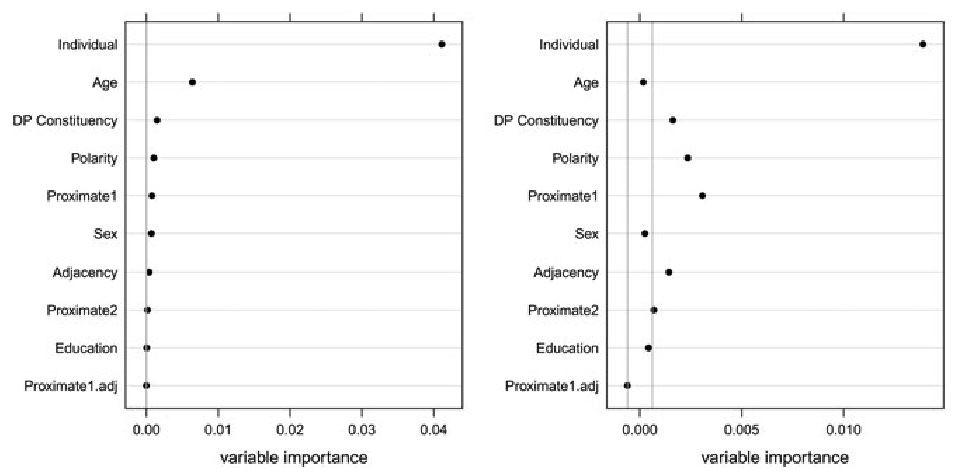
\includegraphics[width = 0.9\linewidth]{images/TagliamonteBaayen_vip.png}
    \caption{Variable importance plot from \citet{tagliamonteModelsForestsTrees2012}. The plot on the left shows the impurity importance (i.e., Gini index) and the plot on the right shows the permutation importance. The y-axis shows the different predictors for both plots.}
    \label{fig:tagliamonte_importance}
\end{figure}

Looking at both the impurity and permutation importance, we can get a better understanding of which predictors are the most important in making the splits in the space. For \citet{tagliamonteModelsForestsTrees2012}, this meant that the Individual variable was the most important predictor in making the splits in the data. The other predictors were also important, but we now see differences between the two plots in which are important. In general, the researcher should look at both the impurity importance and the permutation importance to gain an understanding of which predictors are the most important in making the splits in the data. If there is a overlap between the two plots, then we can be more confident that the predictor is important in making the splits in the data. If there is a large difference between the importance of a predictor between the two plots, then we should be cautious about that predictor's importance. 

%--------------------------
\section{Random Forests in SLZ} \label{sec:bagging_slz}
%--------------------------

In this section, I will present the results of a Random Forest analysis that was performed on the SLZ data. The goal of this analysis is to understand which acoustic measures are the most important in achieving the separations in the acoustic space of the SLZ. The data collection and analysis methods are similar to those used in the MDS analysis presented in Chapter~\ref{ch:acousticlandscape}. The main difference is that I will be using a Random Forests analysis instead of an MDS analysis. The results of this analysis will be presented in the following sections.

%--------------------------------------------------------------------------
\subsection{Methods} \label{sec:methods}
%--------------------------------------------------------------------------
%--------------------------------------------------------------------------
\subsubsection{Participants} \label{sec:participants}
%--------------------------------------------------------------------------
This study uses data collected from 10 native speakers of SLZ during the summer of 2022. Participants were recruited from the community of Santiago Laxopa, Oaxaca, Mexico. All participants were native speakers of SLZ. The participants were between 18 and 60 years old and consisted of five males and five females.

%--------------------------------------------------------------------------
\subsubsection{Recordings} \label{sec:recordings} 
%--------------------------------------------------------------------------
Participants were asked to perform a word list elicitation task consisting of 72 words. These words were selected to elicit the entire range of types of voice quality in SLZ, including modal voice, the two kinds of creaky (i.e., checked and rearticulated), and breathy voice. The words were selected based on previous research conducted as part of the Zapotec Language Project at the University of California, Santa Cruz \citep{ZapotecLanguageProject}. 
Because participants were not literate in SLZ, the word list was prompted for them by asking them ``How do you say [word in Spanish]?" by myself and another researcher in Zapotec. Participants were asked to respond with the desired word in the carrier phrase \textit{Shnia' X chonhe lhas} [ʃnːiaˀ X tʃone ɾas] ``I say X three times.'' which was repeated three times. These utterances were recorded in a quiet environment using a Zoom H4n handheld digital recorder. The recordings were saved as 16-bit WAV files with a sampling rate of 44.1 kHz.

%--------------------------------------------------------------------------
\subsubsection{Acoustic measuring} \label{sec:acoustics}
%--------------------------------------------------------------------------

The resulting audio files were then processed in Praat to isolate the vowel portion of each word. The onset of the vowel was set to the second glottal pulse after the onset, and the offset of the vowel was set to the last glottal pulse before the decrease in amplitude at the end of the vowel \citep{garellekAcousticDiscriminabilityComplex2020}. The vowel was then extracted and saved as a separate file for analysis.

These vowels were fed into VoiceSauce \citep{shueVoiceSauceProgramVoice2011} to generate the acoustic measures for the studies discussed in this dissertation. Because many acoustic measures are based on the fundamental frequency, this measure was calculated using the STRAIGHT algorithm from \citep{kawaharaInstantaneousfrequencybasedPitchExtraction1998} to estimate the fundamental frequency in millisecond (ms) intervals. Once the fundamental frequency is calculated, VoiceSauce then uses an optimization function to locate the harmonics of the spectrum, finding their amplitudes.

VoiceSauce then uses the Snack Sound toolkit \citep{sjolanderSnackSoundToolkit2004} to find the frequencies and bandwidths of the first four formants, also at millisecond intervals. The amplitudes of the harmonics closest to these formant frequencies are located and treated as the amplitudes of the formants. These formant frequencies and bandwidths are used to correct the harmonic amplitudes for the filtering effects of the vocal tract, using \citeauthor{iseliAgeSexVowel2007}'s \citeyear{iseliAgeSexVowel2007} extension of the method employed by \citet{hansonGlottalCharacteristicsFemale1997}. Each vowel was measured across ten equal time intervals, resulting in 22890 data points in total. These measures were then z-scored by speaker to reduce the variation between speakers and provide a way to compare the different measures directly on similar scales.

%--------------------------------------------------------------------------
\subsubsection{Data processing} \label{sec:data_processing}
%--------------------------------------------------------------------------
Data points with an absolute z-score value greater than three were considered outliers and excluded from the analysis. The Mahalanobis distance was calculated in the F1-F2 panel within each vowel category. Each data point with a Mahalanobis distance greater than six was considered an outlier and excluded from the analysis. Using the Mahalanobis distance allows us to compare the data points to the mean of the F1-F2 panel for each vowel category. The larger the Mahalanobis distance is the more deviant the data point is from the mean which in turn means that the data point was improperly tracked. This is comparable to what was done in \citet{seyfarthPlosiveVoicingAcoustics2018,chaiCheckedSyllablesChecked2022,garellekPhoneticsWhiteHmong2023}.

Energy was excluded if it had a zero value and then log-transformed to normalize its right-skewed distribution. Afterward, the resulting log-transformed Energy was z-scored, and any data point with a z-score greater than three was excluded. This outlier removal resulted in 1918 data points being removed. 

All data points were then z-scored by speaker to reduce the variation between speakers and provide a way to compare the different measures directly on the same scale.

Residual H1* for the remaining data points following \citet{chaiH1H2AcousticMeasure2022}. First, a linear mixed effects model was generated with the z-scored H1* as the response variable and the z-scored energy as the fixed effect. The uncorrelated interaction of the z-scored energy by speaker was treated as random. The energy factor resulting from this linear mixed-effects model was extracted. Finally, the z-scored H1* had the product of the z-scored energy and energy factor subtracted from it to produce the residual H1* measure. 

Once these steps were completed, the mean of each combination of phonation and speaker was taken for the fourth to seventh interval of the vowel. This is similar to what \citet{keatingCrosslanguageAcousticSpace2023} did by taking the middle of the vowel for their analysis. This choice minimizes the effect of the onset and offset of the vowel on the acoustic measures, which are more likely to be affected by the surrounding consonants and should give us the most accurate representation of the vowel quality. Because z-scores were used, this resulted in negative measures, which presents a problem for MDS analyses. To correct for this, I added the absolute value of the minimum z-score to each measure. This results in a dataset that still preserves the relative differences in the scores. 
%--------------------------------------------------------------------------
\subsection{Parameter selection} \label{sec:bagging_model}
%--------------------------------------------------------------------------

In order to determine the correct number of trees and the number of predictors to use at each split, I followed the methods outlined in \citet{boehmkeHandsOnMachineLearning2019} and \citet{jamesIntroductionStatisticalLearning2021} for parameter selection. The data was split into a training set and a test set. The training set was used to train the model and the test set was used to evaluate the performance of the model. The training set consisted of 70\% of the data and the test set consisted of 30\% of the data. The split was done so that the distributions of the different voice qualities was the same between the training and test sets. The training set was then used to tune the parameters of the model. The parameters that were tuned were the number of trees, the number of predictors to use at each split, the amount to sample from the training set, and whether to sample with replacement. The values for the parameters were chosen based on the results of a grid search.

Using a grid search allowed me to systematically search through the different combinations of parameters to find the best combination for the model. Another reason was that this allowed me to determine if Bagging (i.e., using all of the predictors at each split) or Random Forests (i.e., using a random subset of the predictors at each split) was the best model for the data. The model whose parameters resulted in the most accurate model was chosen as the final model. 

Figure~\ref{fig:mtry_number}, shows the results of the grid search in relation to the number of trees and the number of predictors to use at each split. The x-axis shows the number of trees that were used in the model and the y-axis shows the percentage of incorrectly classified out-of-bag tokens. The lower the out-of-bag error percentage, the better the model is at predicting unseen data. The colored lines show the different values of $m_{try}$ that were used in the model. When $m_{try} = 22$, the model uses all the predictors in each split and is therefore a bagging model. The other potential values for $m_{try}$ are the values corresponding to 5\%, 15\%, 25\%, and 40\% of the total number of predictors. Furthermore, the default values of $m_{try} = \sqrt{22}$ and $m_{try} = \frac{22}{3}$ for classification and regression trees were considered, these values were recommended by \citet{boehmkeHandsOnMachineLearning2019}. 

Figure~\ref{fig:mtry_number} shows that the model with $m_{try} = 22$ (i.e., bagging) is not the best model for the data. This is because it has a very high percentage of out-of-bag error compared to the other models. The model that performed the best was the model that trained on 300 trees and whose $m_{try} = 5$ had the lowest percentages of out-of-bag errors. Furthermore, it was found that sampling only 80\% of the replacement data produced the best model.\footnote{The full grid search results can be found online at my website: \href{mlbrinkerhoff.me}{mlbrinkerhoff.me}.}

\begin{figure}[h!]
    \centering
    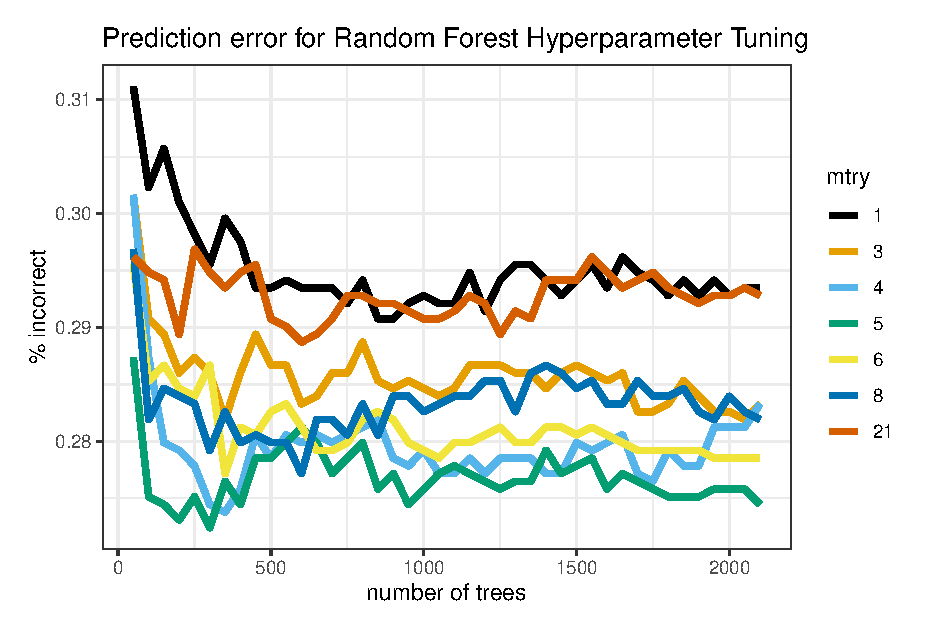
\includegraphics[width = 0.9\linewidth]{images/RandomForest/tree_num_dur.eps}
    \caption{Plot showing the percent of inaccurately classified phonation types as a function of the number of trees ran. The different colored lines indicate the different $m_{try}$ values.}
    \label{fig:mtry_number}
\end{figure}

%--------------------------------------------------------------------------
\section{Results} \label{sec:dt_results}
%--------------------------------------------------------------------------

The results of the Random Forest analysis are shown in Figure~\ref{fig:predictor_importance}. The plot on the left shows the impurity importance which uses the mean decrease in the Gini index to measure the importance of each predictor. The Gini index is a measure of how pure the split is and is calculated for each variable and then averaged across all trees. The higher the Gini index, the more important that variable is in making the splits in the data. The plot on the right shows the permutation importance, which measures the change in the model's prediction accuracy when the values of a variable are randomly permuted (i.e., the variable is shuffled and the model is reevaluated). The difference in accuracy between the original model and the permuted model is then used to measure the importance of that variable. The higher the difference, the more important that variable is in splitting the data. The y-axis shows all 21 different predictors for both plots. However, the predictors in each plot are ranked in descending order of importance. 

\begin{figure}[h!]
    \centering
    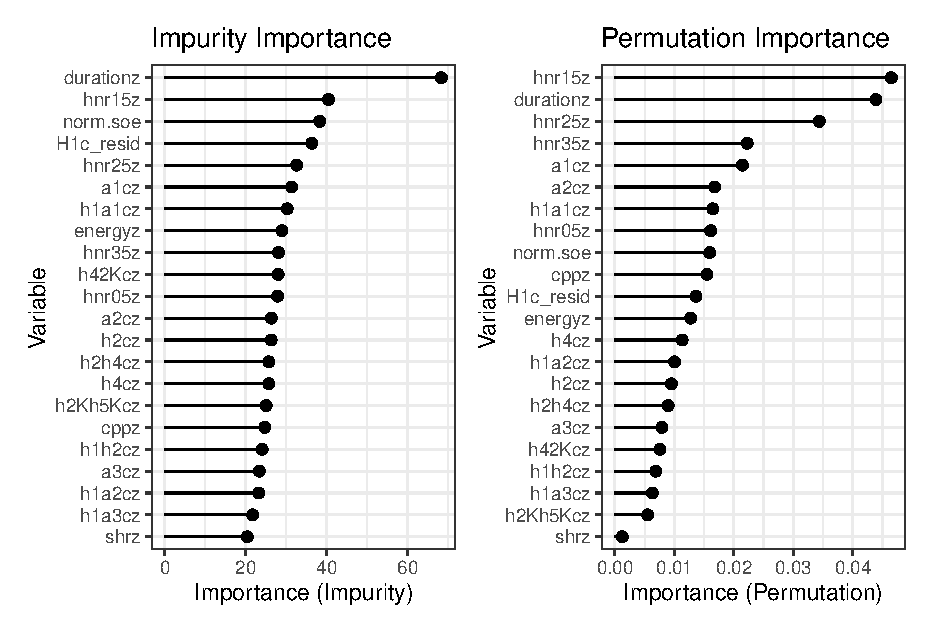
\includegraphics[width = \linewidth]{images/RandomForest/rf_dur_plots.eps}
    \caption{Variable importance plots showing the impurity importance and permutation importance of each acoustic measure.}
    \label{fig:predictor_importance}
\end{figure}

From Figure~\ref{fig:predictor_importance}, we can see that the two most important predictors for classifying the different phonations are: (i) duration and (ii) HNR < 1500 Hz. The reason for this is that both of these measures appear as the two highest predictors in terms of impurity and permutation. Each of the predictors suggested by the model will be discussed in more detail below. 

The rest of the variables require some discussion to determine their importance. This is because the next several predictors in both plots are not consistent. In the impurity importance plot, we see that Strength of Excitation and residual H1* are the next most important measures. However, their importance decreases when we consider permutation. Instead of being the third and fourth most important impurity predictors, they are now the ninth and eleventh most important permutation predictors. Because both measures are sifted only slightly and are in the upper half of both plots, we can assume that these acoustic measures still play an important role to some extent.

Furthermore, we see that A1* is relatively consistent between the two plots. In the impurity plot on the left it is the sixth most important predictor and in the permutation plot on the right it is the fifth most important predictor. This suggests that A1* plays an important role in classifying the different phonations. The same reasoning holds for H1*$-$A1*, which is the seventh most important predictor in both plots. 

%--------------------------
\section{Discussion of the results} \label{sec:dt_discussion}
%--------------------------

This section will discuss the results of the Random Forest analysis in two parts. The first part will discuss the results of the Random Forest analysis in relation to the MDS analysis presented in Chapter~\ref{ch:acousticlandscape}. The second part will discuss certain acoustic measures that were shared by the analyses and those that were uniquely chosen by the Random Forest analysis. 
%--------------------------
\subsection{Comparing the MDS and bagging trees} \label{sec:dt_mds}
%--------------------------
There was a large amount of overlap between which measures were correlated with the dimensions of the MDS analysis and the important predictors found by the Random Forest analysis. The correlations for the MDS analysis were found in Chapter~\ref{ch:acousticlandscape} and are shown in Table~\ref{tab:acoustic_correlates}. They are repeated here as Table~\ref{tab:acoustic_correlates_repeat} for convenience.  

\begin{table}[h!]
    \centering
    \caption{Correlations for each acoustic measure to the four dimensions (NMDS1, NMDS2, NMDS3, NMDS4). The four largest correlations in each dimension are bolded.} 
    \label{tab:acoustic_correlates_repeat}
    \begin{tabular}{lrrrr}
        \lsptoprule
        Acoustic Measure & NMDS1 & NMDS2 & NMDS3 & NMDS4 \\ 
        \hline
        H1*$-$H2* & -0.221 & -0.339 & 0.031 & 0.314 \\ 
        H2*$-$H4 & -0.437 & 0.239 & \textbf{-0.689} & \textbf{-0.364} \\ 
        H1*$-$A1* & \textbf{-0.828} & 0.048 & \textbf{-0.459} & 0.044 \\ 
        H1*$-$A2* & \textbf{-0.855} & -0.067 & -0.343 & 0.114 \\ 
        H1*$-$A3* & \textbf{-0.809} & -0.218 & -0.297 & 0.126 \\ 
        H4*$-$H2k* & -0.452 & -0.598 & 0.294 & \textbf{0.366} \\ 
        H2k*$-$H5k* & 0.152 & 0.023 & 0.101 & 0.057 \\ 
        residual H1* & -0.290 & -0.443 & \textbf{-0.722} & 0.084 \\ 
        H2* & -0.157 & -0.555 & \textbf{-0.679} & 0.114 \\ 
        H4* & 0.295 & \textbf{-0.778} & 0.078 & \textbf{0.479} \\ 
        A1* & 0.756 & -0.549 & 0.092 & 0.124 \\ 
        A2* & \textbf{0.779} & -0.476 & -0.103 & 0.086 \\ 
        A3* & 0.735 & -0.416 & -0.211 & 0.093 \\ 
        CPP & -0.590 & -0.606 & 0.209 & -0.179 \\ 
        HNR < 500 Hz & -0.513 & \textbf{-0.792} & 0.152 & -0.202 \\ 
        HNR < 1500 Hz & -0.275 & \textbf{-0.799} & 0.323 & -0.290 \\ 
        HNR < 2500 Hz & -0.327 & -0.714 & 0.391 & -0.348 \\ 
        HNR < 3500 Hz & -0.446 & -0.644 & 0.393 & -0.356 \\ 
        Strength of Excitation & -0.013 & -0.741 & -0.238 & 0.145 \\ 
        SHR & 0.144 & -0.176 & 0.122 & \textbf{-0.597} \\ 
        Energy & -0.080 & \textbf{-0.793} & -0.015 & 0.341 \\ 
        Duration & -0.622 & 0.539 & 0.257 & 0.030 \\ 
        \lspbottomrule
    \end{tabular}
\end{table}

The rest of this section will discuss each of the measures where there was overlap between which measures showed a correlation to a MDS dimension and the Random Forest results. Furthermore, I will discuss duration and A1* due to how important the Random Forest model showed these measures. These measures are: (i) duration, (ii) A1*, (iii) H1*$-$A1*, (iv)  residual H1*, (v) HNR < 1500 Hz, and (vi) Strength of Excitation. Each of these measures will be discussed in the following subsections in the order described above.

%--------------------------
\subsection{Importance of duration} \label{sec:duration_discussion}
%--------------------------
In the Random Forest analysis, duration was found to be one of the most important predictors in classifying the different phonations. This importance is reflected in the fact that it is the most important predictor in the impurity importance plot and the second most important predictor in the permutation importance plot. 

Duration frequently plays an important role in Zapotec phonation contrasts. Many descriptions of Zapotec languages have shown that duration is often an important correlate for checked vowels \citep{ariza-garciaPhonationTypesTones2018}. This has also been reported by \citet{chaiPerceptionCheckedRearticulated2025} for Yateé Zapotec, a variety of Zapotec spoken in the Sierra Norte region of Oaxaca, Mexico, and a close relative of SLZ. \citet{chaiPerceptionCheckedRearticulated2025} found that duration was the most important percept for distinguishing between Yateé Zapotec's checked and rearticulated vowels. \citeauthor{chaiPerceptionCheckedRearticulated2025} also found that the longer the duration of the vowel, the more likely the speakers of Yateé Zapotec were to classify the vowel as rearticulated. Similar results for checked vowels have been reported for other Zapotec varieties \citep{arellanesarellanesSistemaFonologicoPropiedades2009,arellanesarellanesDosGradosLaringizacion2010,chavez-peonInteractionMetricalStructure2010,lopeznicolasEstudiosFonologiaGramatica2016,merrillTilquiapanZapotec2008}, other members of the Oto-Manguean family \citep[e.g.,][]{campbellAspectsPhonologyMorphology2014}, and crosslinguistically \citep{gaoPhonationVariationFunction2022,chaiCheckedSyllablesChecked2022}. 

In their study on contextual enhancement effects on phonation contrasts in San Pablo Macuiltianguis Zapotec, \citet{barzilaiContextdependentPhoneticEnhancement2021} found that duration played a role in distinguishing between the different types of phonation, regardless of the phrasal context. They found that modal vowels were the longest and checked vowels the shortest. In regards to rearticulated vowels, they claim that they do not function as a separate phonation type but rather are a sequence of a checked vowel followed by a modal vowel. Despite this reanalysis, we would then expect the duration of the rearticulated vowel to be longer, given that they are a sequence of two vowels. 

In SLZ, the duration distribution between the different phonation types is shown in Figure~\ref{fig:duration_plot}. The y-axis shows the duration of each of the different phonation types in z-scores, again, z-scores were used to minimize individual speaker variation. The x-axis shows each of the four different phonations. The plot shows that the breathy voice has the longest duration and the rearticulated voice has the longest duration, followed by the checked voice. The shortest duration is found in the modal voice. 

\begin{figure}[h!]
    \centering
    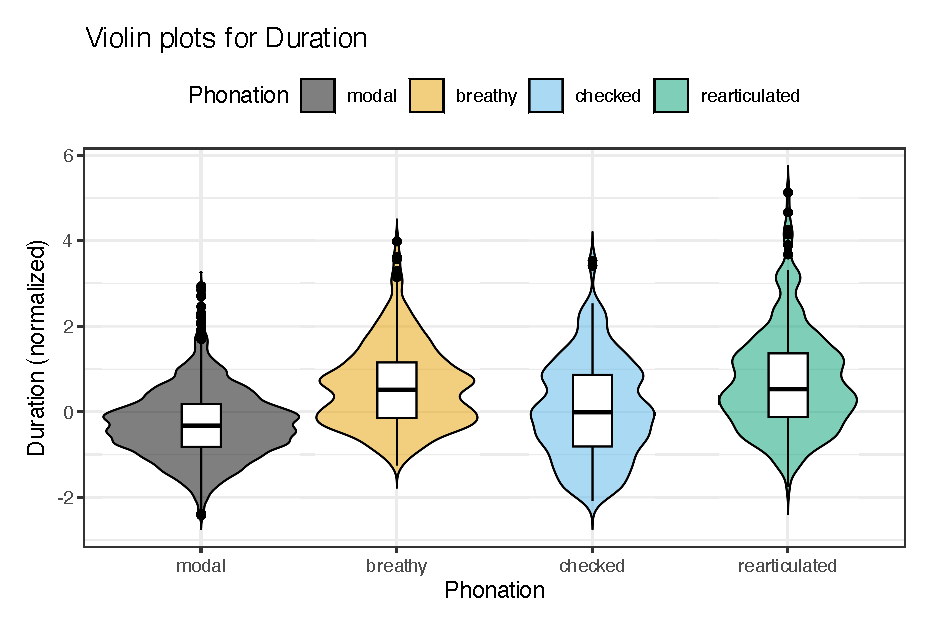
\includegraphics[width = 0.9\linewidth]{images/duration_plot.eps}
    \caption{Plot showing the distribution of duration across the different voice qualities in SLZ.}
    \label{fig:duration_plot}
\end{figure}

These results are somewhat surprising because of the generalization that checked vowels are vowels that are abruptly stopped at the end of the vowel. This is not the case in SLZ. The checked vowels in SLZ are indeed the shortest of the three non-modal phonations. However, they are not the shortest when modal is included. This is likely due to the fact that checked vowels are often limited to final open word syllables in SLZ, and there is a general trend in Zapotec phonology for these syllables to be longer or minimally bimoraic \citep[e.g.,][]{,chavez-peonInteractionMetricalStructure2010,nellisFortisLenisCajonos1980,uchiharaFortisLenisGlides2016}. 

When we consider the behavior of nonmodal phonation cross-linguistically, we see that the behavior of duration is consistent with what is generally found. For example, \citet{gordonPhonationTypesCrosslinguistic2001,espositoCrosslinguisticPatternsPhonation2020} both report that non-modal voice qualities are typically longer than modal voice. One of the reasons for this is that by lengthening the vowel, the speaker is able to increase the amount of time that the glottal source is able to produce the desired voice quality, which increases the likelihood that the listener will be able to perceive the desired voice quality. 

The behavior of duration warrants further investigation in SLZ. If checked vowels are indeed longer than modal vowels, then this would suggest that the checked vowels in SLZ are not the same as the checked vowels in other Zapotec languages. Furthermore, vowels have been claimed to undergo a process of vowel lengthening in Zapotec languages depending on the type of syllable it is in and whether the coda is a fortis or lenis consonant \citep{nellisFortisLenisCajonos1980,uchiharaFortisLenisGlides2016}. 

If the vowel is in an open syllable or a closed syllable with a lenis coda, then the vowel is lengthened. If the vowel is in a closed syllable with a fortis coda, then the vowel is not lengthened. If this behavior is true for SLZ, this means that the duration of the vowel depends not only on the type of phonation but also on the type of syllable in which it is placed. This requires further investigation to determine if the duration is affected by the phonation and type of syllable.
%--------------------------
\subsection{Importance of A1*} \label{sec:a1_discussion}
%--------------------------

The measure that was found to be the most important for classifying the SLZ phonation contrasts was A1*. This measure captures the amplitude of the harmonic closest to the first formant. This measure is typically not found in voice quality research except as a way to normalize the amplitude of the first harmonic (i.e., H1*). This goes back to \citet{fischer-jorgensenPhoneticAnalysisBreathy1968} who used this as one of the ways to correct for the high-pass filtering, in addition to the widely used H1*$-$H2* measure. However, A1* as a standalone measure is not typically used in voice quality research. Therefore, what we are to make of this measure's importance in SLZ is not clear as is its behavior in regards to the different phonations. 

When we look at how A1* is distributed across the different voice qualities in SLZ, as seen in Figure~\ref{fig:a1}, we see that the modal vowels are found at the top of the chart with the other phonation contrasts located lower on the chart. The phonation that is found at the bottom of the chart is a breathy voice. 
\begin{figure}[h!]
    \centering
    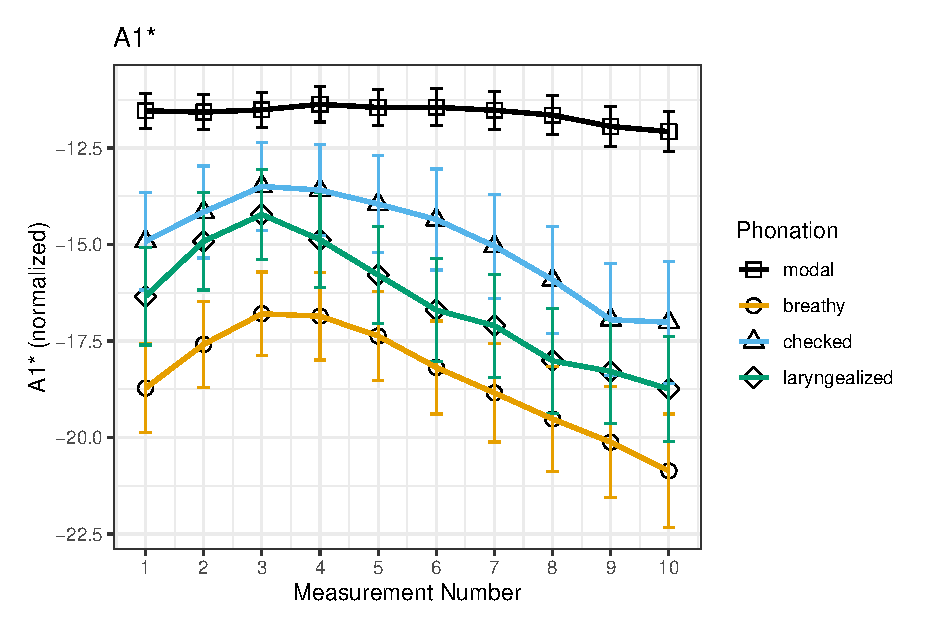
\includegraphics[width = 0.9\linewidth]{images/slz_a1c.eps}
    \caption{Plot showing the distribution of A1* across the different voice qualities in SLZ.}
    \label{fig:a1}
\end{figure}

The pattern of behavior for A1* is very similar to what is found in descriptions of the behavior of the frequency of F1 in breathy voice contexts. For example, differences in the frequency of F1 are typically used to distinguish register differences in Southeast Asian languages \citep{brunelleRegisterEasternCham2005,brunelleDialectExperiencePerceptual2012,brunelleTonePhonationSoutheast2016}.

As described in \citet{brunelleTonePhonationSoutheast2016}, many of the languages of Southeast Asia have what is called register. The linguistic term register is defined as ``the redundant use of pitch, voice quality, vowel quality, and durational differences to distinguish (typically two) contrastive categories'' \citep[193]{brunelleTonePhonationSoutheast2016}, and was first used by \citet{hendersonMainFeaturesCambodian1952} to describe the categorical contrasts found in Khmer. The characteristics that define the higher and lower registers are found in Table~\ref{tab:register_correlates}.

\begin{table}[h!]
    \centering
    \caption{Possible phonetic correlates of register. From \citet{brunelleTonePhonationSoutheast2016}.}
    \label{tab:register_correlates}
    \begin{tabular}{ll}
        \lsptoprule
        \textbf{Higher Register} & \textbf{Lower Register} \\
        \hline
        Higher pitch & Lower pitch \\
        Tense/Modal voice & Lax/Breathy voice \\
        Monophthongs/shorter vowels & Diphthongs/longer vowels \\
        Raised F1/lower vowels/[+ATR] & Lowered F1/higher vowels/[-ATR] \\
        Plain stops/shorter VOT & Aspirated stops/longer VOT \\
        \lspbottomrule
    \end{tabular}
\end{table}

From this table, the lower register is what interests us here. The lower register is associated with breathy voice and a lowered first formant. There is evidence that breathy voice frequently has a lower first formant than modal voice in paralinguistic settings for English \citep{lottoEffectVoiceQuality1997}.  However, these studies do not discuss the amplitude of the first formant but rather the frequency of the first formant.

Another comparison can be found in the research on nasality, where this measure is discussed extensively either alone or in association with the nasal pole (e.g., \cite{chenAcousticCorrelatesEnglish1997,delvauxPerceptionContrasteNasalite2009,macmillanIntegralityNasalizationF11999,pruthiAcousticParametersAutomatic2004,,schwartzAcousticsNormalNasal1968,stevensAcousticPhonetics2000,stylerAcousticalPerceptualFeatures2015,stylerAcousticalFeaturesVowel2017}). These studies discuss how in nasalized contexts the amplitude of the first formant is typically found to be lower than in oral contexts, again similar to what we see in Figure~\ref{fig:a1}.

There is a large body of research that discusses that nasality is closely associated with breathy voice or glottal consonants, in a phenomenon called \textit{rhinoglottophilia} \citep{matisoffRhinoglottophiliaMysteriousConnection1975,ohalaPhoneticExplanationsNasal1975,ohalaPhoneticsNasalPhonology1993,bennettMayanPhonology2016}. In \citet{blevinsEvolutionPonapeicNasal1993,matisoffRhinoglottophiliaMysteriousConnection1975}, this association is attributed to the acoustic and perceptual similarities between nasalization and breathy voice. In one study, \citet{garellekBreathyVoiceNasality2016} showed that nasalization in three different Yi languages was associated with a slender voice. The authors suggested that breathy voice during nasalization can arise from misperception or as a type of phonetic enhancement. 

In terms of what is going on in SLZ, it is not clear if the lowering of A1* for breathy voice can be attributed to the same observations as discussed above. I suggest that there are three different possibilities to explain what is going on in SLZ. First; because SLZ does not have phonemic nasalization, it is possible that speakers of SLZ are using nasalization as a way to phonetically enhance the contrast of breathy voice. Essentially, the reverse of what was reported by \citet{garellekBreathyVoiceNasality2016}. This possibility could be tested acoustically by performing an experiment to detect nasal airflow during breathy vowels. The second possibility is that the same measures that work for detecting nasality can also be used to detect breathy voice. This second possibility could be easily tested by examining whether A1* and the other measures for nasality work in other breathy voice contexts cross-linguistically. The third possibility is that the lowering of A1* is a result of subglottal resonances, which is much harder to test than the other two possibilities. 

%--------------------------
\subsection{Importance of \texorpdfstring{H1*$-$A1*}{H1*-A1*}} \label{sec:h1a1_discussion}
%--------------------------

The Random Forest analysis found H1*$-$A1* to be one of the most important predictors in classifying the different phonations. This is because of its high ranking in both the impurity and permutation importance plots. In the impurity plot, it is the seventh most important predictor, and in the permutation plot, it is the sixth most important predictor.

The acoustic measure H1*$-$A1* is a measure of the difference between the amplitude of the first harmonic and the amplitude of the harmonic closest to the first formant. This acoustic measure falls into the category of spectral slope measures. As discussed in Chapter~\ref{ch:residual_h1}, these measures capture the differences in the amplitude of the harmonics of the spectrum. The higher the values of the spectral slopes, the more breathy the phonation is \citep{fischer-jorgensenPhoneticAnalysisBreathy1968}. The lower the spectral slope values, the more creaky the phonation is.

The distribution of H1*$-$A1* across the different phonation types is shown in Figure~\ref{fig:h1a1}. The y-axis is the z-scored H1*$-$A1* values and the x-axis shows the ten equally spaced intervals throughout the duration of the vowel. 

\begin{figure}[h!]
    \centering
    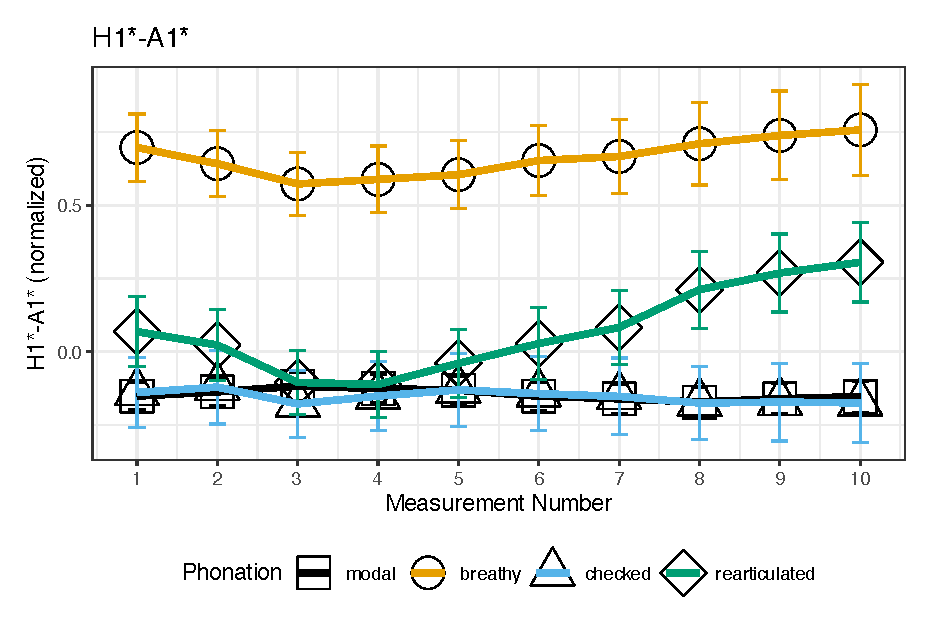
\includegraphics[width = 0.9\linewidth]{images/h1a1_line.eps}
    \caption{Plot showing the distribution of H1*$-$A1* across the different voice qualities in SLZ. Each point represents the mean of the ten equally spaced intervals across the duration of the vowel and the error bars represent a 95\% confidence interval.}
    \label{fig:h1a1}
\end{figure}

The plot shows that breathy voice has the highest H1*$-$A1* score, which is consistent with what we would expect from a spectral slope measure. Things are more complicated when we look at the other non-modal phonations. It is expected that checked voice and rearticulated voice have a lower spectral slope than modal voice because of their association with creaky voice. However, this is not the case in Figure~\ref{fig:h1a1}. 

The plot shows that the checked voice has a spectral slope that is identical to that of the modal voice. Additionally, we see that the rearticulated voice has a spectral slope that is higher than the modal voice except at measurement intervals three and four, where it is identical to the modal voice. This behavior for a rearticulated voice is not too surprising, especially at the end of the vowel. 

One reason for this is that when listening to the rearticulated vowels, the portion of the vowel after the glottal occlusion sounds somewhat breathy. One of the possible explanations for this is that in order to produce the glottal occlusion, the speaker is tightly constricting the vocal folds, which causes either a glottal stop or creaky voice. The speaker then relaxes the vocal folds in order to produce the modal voice which stereotypically occurs after this glottal occlusion. However, one way for the speaker to quickly relax the vocal folds is to open them as much as possible to reach the ideal position for the modal voice. This general behavior of opening the vocal folds to produce a modal voice is similar to what is found in a breathy voice. This could be a possible explanation for why the rearticulated voice has a higher H1*$-$A1* score than modal voice.

%--------------------------
\subsection{Importance of Residual H1*} \label{sec:rh1_discussion}
%--------------------------

Another spectral slope measure that was found to be important in the Random Forest and MDS analyses was residual H1*. This measure is similar to H1*$-$A1* in that it captures the differences in the amplitude of the harmonic of the spectrum. However, residual H1* is a measure that is calculated after removing the effect of energy on H1*. 

As residual H1* is a type of spectral slope measure, it is expected to show similar behavior to other spectral slope measures. That is, a breathy voice should be associated with a higher score than a modal voice. Since the two types of laryngealization are closely associated with creaky voice, they should be associated with a lower score than modal voice. Additionally, there is a temporal difference between the two types of laryngealization, it is expected that checked voice will have a lower score toward the end of the vowel and rearticulated voice will have a lower score in the middle of the vowel. 

In Figure~\ref{fig:residualH1}, we see that the predictions are correct. Breathy voice is associated with a higher score than the modal voice. The two types of laryngealization are associated with a lower score than the modal voice.

\begin{figure}[h!]
    \centering
    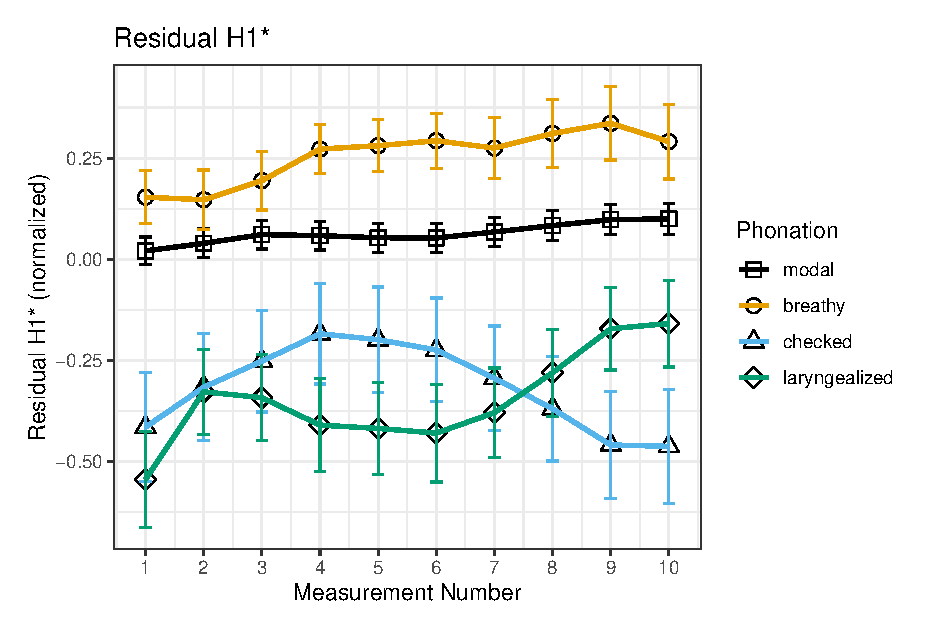
\includegraphics[width = 0.9\linewidth]{images/slz_residual_h1c.eps}
    \caption{Plot showing the distribution of residual H1* across the different voice qualities in SLZ.}
    \label{fig:residualH1}
\end{figure}

A further analysis of the results of this measure using generalized additive (mixed) models (GAM(M)s; \cite{hastieGeneralizedAdditiveModels1986,woodGeneralizedAdditiveModels2017,soskuthyGeneralisedAdditiveMixed2017,wielingAnalyzingDynamicPhonetic2018}) shows that the temporal behavior of the two types of laryngealization is also correct. Checked voice is associated with a lower score toward the end of the vowel, and rearticulated voice is associated with a lower score in the middle of the vowel. Additionally, the results of the GAMM show that for the first three time points there is no significant difference between the breathy and modal voice. The suggestion is that the breathy voice is more closely associated with the latter part of the vowel than with the beginning. The full results of the GAMM for residual H1* are discussed in Chapter~\ref{ch:residual_h1}.

%--------------------------
\subsection{Importance of the HNR \textless 1500 Hz} \label{sec:bagging_hnr}
%--------------------------

The acoustic measure HNR $<$ 1500 Hz is a harmonics-to-noise ratio measure that is calculated over the frequency range from 0 Hz to 1500 Hz and is a measure of the amount of noise in the signal, or in other words, it is a measure of periodicity. In these measures, modal voice is associated with a higher score than nonmodal phonations. This is because modal voice is associated with a higher degree of periodicity than nonmodal phonations because a-periodicity is a defining feature of nonmodal phonations (e.g., \cite{hillenbrandAcousticCorrelatesBreathy1996,blankenshipTimeCourseBreathiness1997,kentVoiceQualityMeasurement1999}).

As seen in Figure~\ref{fig:hnr1500}, this is exactly what we see in SLZ. Modal voice is associated with a higher score than non-modal phonations. Among nonmodal phonations, breathy and rearticulated voice have a higher HNR $<$ 1500 Hz than checked voice. 

\begin{figure}[h!]
    \centering
    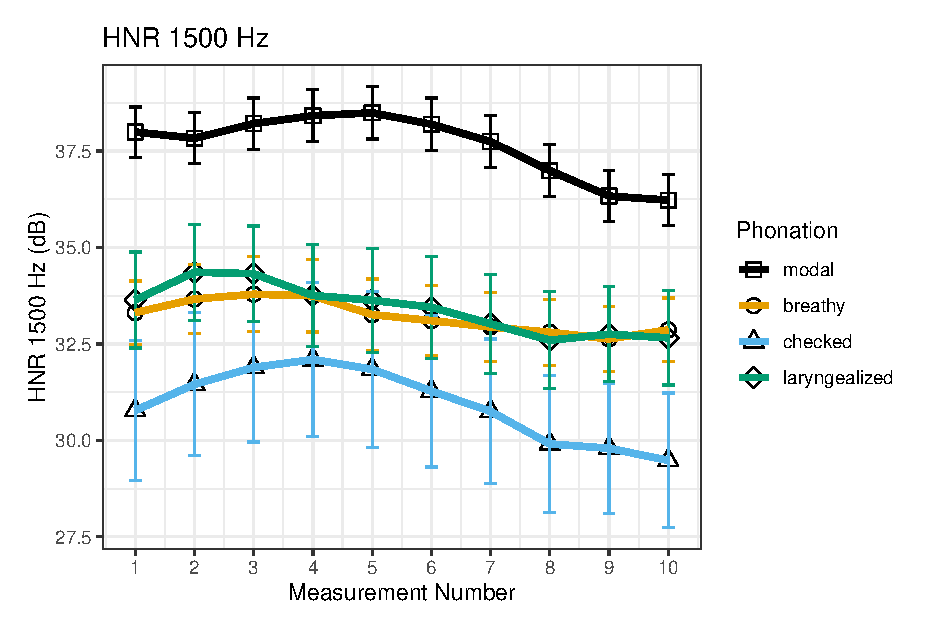
\includegraphics[width = 0.9\linewidth]{images/slz_hnr15.eps}
    \caption{Plot showing the distribution of HNR $<$ 1500 Hz across the different voice qualities in SLZ.}
    \label{fig:hnr1500}
\end{figure}

The fact that breathy and rearticulated voice has a higher HNR $<$ 1500 Hz than checked voice is not surprising. As discussed in Chapter~\ref{ch:SLZ}, rearticulated and breathy voices are associated with more modal-like qualities than checked voice. In most instances of rearticulated voice, the vowel is produced with modal voice except for a small portion of the middle of the vowel where the vowel is produced with creaky voice or a glottal occlusion. Breathy voice typically appears very periodic but with a high degree of noise in the signal. Checked voice on the other hand, is associated with a high degree of aperiodic voicing in the signal from the creaky voice that is produced at the end of the vowel. This is why checked voice has the lowest HNR $<$ 1500 Hz of nonmodal phonations.

This measure will be very important in Chapter~\ref{ch:testing_lc}, where I will use it to model laryngeal complexity.

%--------------------------
\subsection{Importance of Strength of Excitation} \label{sec:dt_soe}
%--------------------------

Strength of Excitation (SoE) is a measure that is defined as ``the instant of significant excitation of the vocal-tract system during production of speech [and represents] the relative amplitude of impulse-like excitation'' \citep[1934]{mittalStudyEffectsVocal2014}. This measure is typically associated with the amplitude of the voicing, or in other words, the degree of voicing during production \citep{murtyEpochExtractionSpeech2008,mittalStudyEffectsVocal2014}. This measure has been shown to be an effective measure for showing the effects of laryngealization on the amplitude of voicing \citep{garellekVoicingGlottalConsonants2021} and has been shown to be effective in distinguishing the different phonations in the Oto-Manguean languages \citep{chaiPhoneticsGlottalizedPhonations2023,wellerInteractionsToneGlottalization2023,wellerLexicalToneVowel2023,wellerVoiceQualityTone2024}.

Following \citet{garellekVoicingGlottalConsonants2021}, it is expected that the modal voice will have the highest SoE score. It is also expected that, because the breathy, rearticulated, and checked voice will have a lower SoE score. The reason for this expectation is that according to \citet{garellekVoicingGlottalConsonants2021}, there is a strong tendency for all types of laryngealization to have a dampening effect on voicing. This is evidenced by the lower SoE scores for these phonations. The score for SoE ranges from 0 to 1, where 0 is no voicing and 1 is full voicing. 

In Figure~\ref{fig:soe}, we observe that the modal voice has the highest SoE score. The three non-modal phonations are all lower. We can ignore the SoE values at measurement numbers one and ten because they represent the beginning and end of the vowel and are more likely to be affected by the coarticulatory effects of the surrounding consonants. However, we can see that breathy voice has a higher SoE score than checked voice and rearticulated voice. Additionally, we see that between checked and rearticulated voice, we see that checked voice has a higher SoE score in the first half of the vowel and rearticulated voice has a higher SoE score in the second half of the vowel. This is consistent with what we would expect from the behavior of the phasing difference between checked and rearticulated vowels. 

\begin{figure}[h!]
    \centering
    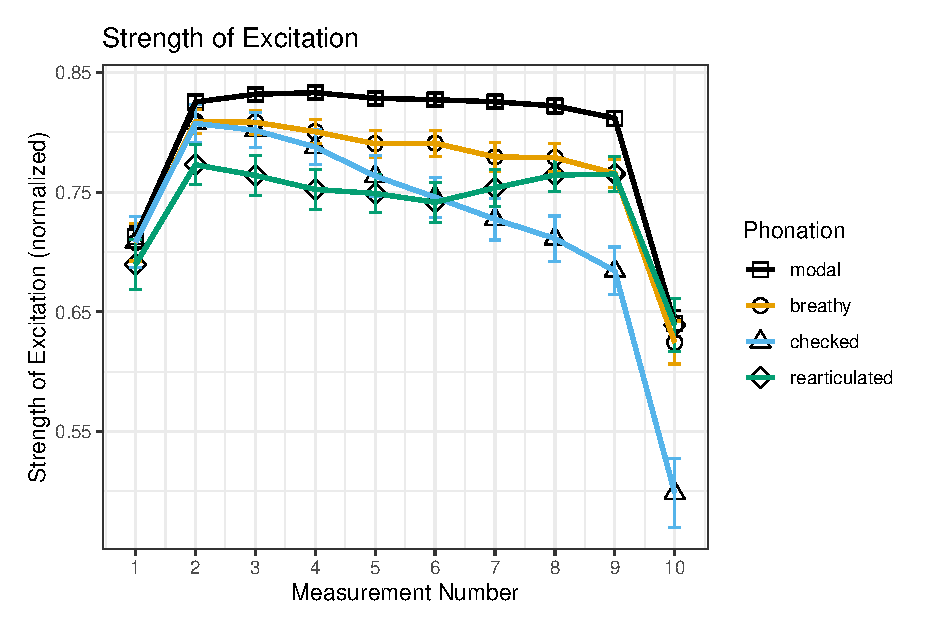
\includegraphics{images/slz_soe.eps}
    \caption{Plot showing the distribution of Strength of Excitation across the different voice qualities in SLZ.}
    \label{fig:soe}
\end{figure}

One thing to note about the SoE measures is that even though nonmodal phonations are associated with a lower SoE score than modal voice, the values for these measures are still extremely high. This likely indicates that even though laryngealization is present in these phonations, the speakers are only weakly laryngealizing the vowel. This is consistent with the claims made by \citet{silvermanLaryngealComplexityOtomanguean1997,silvermanPhasingRecoverability1997} that laryngeally complex languages that do not show a phasing relationship between modal and non-modal phonation must weakly produce non-modal phonation. The claims about laryngeal complexity will be discussed in more detail in Chapter~\ref{ch:testing_lc}.

%--------------------------
\section{Conclusion} \label{sec:dt_conclusion}
%--------------------------


In summary, we find that the results of the Random Forest and the MDS analyses showed a lot of overlap between which measures were correlated and/or important for classifying SLZ's four phonation types. In both analyses, A1*, H1*$-$A1*, residual H1*, HNR $<$ 1500 Hz, and SoE were found to be important acoustic measures. We saw that each of these measures was able to capture some aspect of the phonation types. It also shows that the spectral slope measures and harmonics-to-noise ratio measures are generally the most important measures for classifying the different phonation types. This is consistent with previous work on the acoustics of phonation \citep[e.g.,][]{garellekPhoneticsVoice2019}. We also saw that SoE plays an important role in classifying the different phonation types. This contributes to the growing body of literature that shows that SoE is an important measure for classifying the different phonation types \citep{chaiPhoneticsGlottalizedPhonations2023,garellekVoicingGlottalConsonants2021,wellerInteractionsToneGlottalization2023,wellerLexicalToneVowel2023,wellerVoiceQualityTone2024}.

Interestingly, the results of the Random Forest analysis showed that duration was the most important predictor in classifying the different phonations. This is consistent with what has been found in other Zapotec languages \citep[e.g.,][]{barzilaiContextdependentPhoneticEnhancement2021,chaiPerceptionCheckedRearticulated2025,chavez-peonInteractionMetricalStructure2010}. However, when we plotted the duration, it showed that modal vowels had the shortest duration instead of checked vowels having the shortest duration. The effect of duration needs to be further investigated in SLZ, especially with respect to differences in syllable type and the claimed effects of vowel lengthening in the various Zapotec languages \citep[e.g.,][]{chavez-peonInteractionMetricalStructure2010,merrillTilquiapanZapotec2008,nellisFortisLenisCajonos1980,pickettIsthmusJuchitanZapotec2010,uchiharaFortisLenisGlides2016}.




